\chapter{Number theory}

\index{number theory}

\key{Number theory} is a branch of mathematics
that studies integers.
Number theory is a fascinating field,
because many questions involving integers
are very difficult to solve even if they
seem simple at first glance.

As an example, let us consider the following equation:
\[x^3 + y^3 + z^3 = 33\]
It is easy to find three real numbers $x$, $y$ and $z$
that satisfy the equation.
For example, we can choose
\[
\begin{array}{lcl}
x = 3, \\
y = \sqrt[3]{3}, \\
z = \sqrt[3]{3}.\\
\end{array}
\]
However, nobody knows if there are any three
\emph{integers} $x$, $y$ and $z$
that would satisfy the equation, but this
is an open problem in number theory.

In this chapter, we will focus on basic concepts
and algorithms in number theory.
Throughout the chapter, we will assume that all numbers
are integers, if not otherwise stated.

\section{Primes and factors}

\index{divisibility}
\index{factor}
\index{divisor}

A number $a$ is a \key{factor} or \key{divisor} of a number $b$
if $a$ divides $b$.
If $a$ is a factor of $b$,
we write $a \mid b$, and otherwise we write $a \nmid b$.
For example, the factors of the number 24 are
1, 2, 3, 4, 6, 8, 12 and 24.

\index{prime}
\index{prime decomposition}

A number $n>1$ is a \key{prime}
if its only positive factors are 1 and $n$.
For example, the numbers 7, 19 and 41 are primes.
The number 35 is not a prime, because it can be
divided into the factors $5 \cdot 7 = 35$.
For each number $n>1$, there is a unique
\key{prime factorization}
\[ n = p_1^{\alpha_1} p_2^{\alpha_2} \cdots p_k^{\alpha_k},\]
where $p_1,p_2,\ldots,p_k$ are primes and
$\alpha_1,\alpha_2,\ldots,\alpha_k$ are positive numbers.
For example, the prime factorization for the number 84 is
\[84 = 2^2 \cdot 3^1 \cdot 7^1.\]

The \key{number of factors} of a number $n$ is
\[\tau(n)=\prod_{i=1}^k (\alpha_i+1),\]
because for each prime $p_i$, there are
$\alpha_i+1$ ways to choose how many times
it appears in the factor.
For example, the number of factors
of the number 84 is
$\tau(84)=3 \cdot 2 \cdot 2 = 12$.
The factors are
1, 2, 3, 4, 6, 7, 12, 14, 21, 28, 42 and 84.

The \key{sum of factors} of $n$ is
\[\sigma(n)=\prod_{i=1}^k (1+p_i+\ldots+p_i^{\alpha_i}) = \prod_{i=1}^k \frac{p_i^{a_i+1}-1}{p_i-1},\]
where the latter formula is based on the geometric progression formula.
For example, the sum of factors of the number 84 is
\[\sigma(84)=\frac{2^3-1}{2-1} \cdot \frac{3^2-1}{3-1} \cdot \frac{7^2-1}{7-1} = 7 \cdot 4 \cdot 8 = 224.\]

The \key{product of factors} of $n$ is
\[\mu(n)=n^{\tau(n)/2},\]
because we can form $\tau(n)/2$ pairs from the factors,
each with product $n$.
For example, the factors of the number 84
produce the pairs
$1 \cdot 84$, $2 \cdot 42$, $3 \cdot 28$, etc.,
and the product of the factors is $\mu(84)=84^6=351298031616$.

\index{perfect number}

A number $n$ is \key{perfect} if $n=\sigma(n)-n$,
i.e., $n$ equals the sum of its factors
between $1$ and $n-1$.
For example, the number 28 is perfect,
because $28=1+2+4+7+14$.

\subsubsection{Number of primes}

It is easy to show that there is an infinite number
of primes.
If the number of primes would be finite,
we could construct a set $P=\{p_1,p_2,\ldots,p_n\}$
that would contain all the primes.
For example, $p_1=2$, $p_2=3$, $p_3=5$, and so on.
However, using $P$, we could form a new prime
\[p_1 p_2 \cdots p_n+1\]
that is larger than all elements in $P$.
This is a contradiction, and the number of primes
has to be infinite.

\subsubsection{Density of primes}

The density of primes means how often there are primes
among the numbers.
Let $\pi(n)$ denote the number of primes between
$1$ and $n$. For example, $\pi(10)=4$, because
there are 4 primes between $1$ and $10$: 2, 3, 5 and 7.

It is possible to show that
\[\pi(n) \approx \frac{n}{\ln n},\]
which means that primes are quite frequent.
For example, the number of primes between
$1$ and $10^6$ is $\pi(10^6)=78498$,
and $10^6 / \ln 10^6 \approx 72382$.

\subsubsection{Conjectures}

There are many \emph{conjectures} involving primes.
Most people think that the conjectures are true,
but nobody has been able to prove them.
For example, the following conjectures are famous:

\begin{itemize}
\index{Goldbach's conjecture}
\item \key{Goldbach's conjecture}:
Each even integer $n>2$ can be represented as a
sum $n=a+b$ so that both $a$ and $b$ are primes.
\index{twin prime}
\item \key{Twin prime conjecture}:
There is an infinite number of pairs
of the form $\{p,p+2\}$,
where both $p$ and $p+2$ are primes.
\index{Legendre's conjecture}
\item \key{Legendre's conjecture}:
There is always a prime between numbers
$n^2$ and $(n+1)^2$, where $n$ is any positive integer.
\end{itemize}

\subsubsection{Basic algorithms}

If a number $n$ is not prime,
it can be represented as a product $a \cdot b$,
where $a \le \sqrt n$ or $b \le \sqrt n$,
so it certainly has a factor between $2$ and $\lfloor \sqrt n \rfloor$.
Using this observation, we can both test
if a number is prime and find the prime factorization
of a number in $O(\sqrt n)$ time.

The following function \texttt{prime} checks
if the given number $n$ is prime.
The function attempts to divide $n$ by
all numbers between $2$ and $\lfloor \sqrt n \rfloor$,
and if none of them divides $n$, then $n$ is prime.

\begin{lstlisting}
bool prime(int n) {
    if (n < 2) return false;
    for (int x = 2; x*x <= n; x++) {
        if (n%x == 0) return false;
    }
    return true;
}
\end{lstlisting}

\noindent
The following function \texttt{factors}
constructs a vector that contains the prime
factorization of $n$.
The function divides $n$ by its prime factors,
and adds them to the vector.
The process ends when the remaining number $n$
has no factors between $2$ and $\lfloor \sqrt n \rfloor$.
If $n>1$, it is prime and the last factor.

\begin{lstlisting}
vector<int> factors(int n) {
    vector<int> f;
    for (int x = 2; x*x <= n; x++) {
        while (n%x == 0) {
            f.push_back(x);
            n /= x;
        }
    }
    if (n > 1) f.push_back(n);
    return f;
}
\end{lstlisting}

Note that each prime factor appears in the vector
as many times as it divides the number.
For example, $24=2^3 \cdot 3$,
so the result of the function is $[2,2,2,3]$.

\subsubsection{Sieve of Eratosthenes}

\index{sieve of Eratosthenes}

The \key{sieve of Eratosthenes} is a preprocessing
algorithm that builds an array using which we
can efficiently check if a given number between $2 \ldots n$
is prime and, if it is not, find one prime factor of the number.

The algorithm builds an array $\texttt{a}$
whose positions $2,3,\ldots,n$ are used.
The value $\texttt{a}[k]=0$ means
that $k$ is prime,
and the value $\texttt{a}[k] \neq 0$
means that $k$ is not a prime and one
of its prime factors is $\texttt{a}[k]$.

The algorithm iterates through the numbers
$2 \ldots n$ one by one.
Always when a new prime $x$ is found,
the algorithm records that the multiples
of $x$ ($2x,3x,4x,\ldots$) are not primes,
because the number $x$ divides them.

For example, if $n=20$, the array is as follows:

\begin{center}
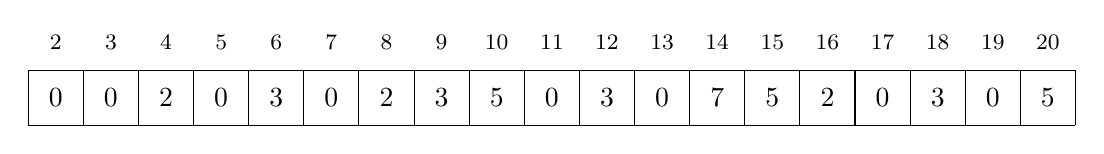
\begin{tikzpicture}[scale=0.7]
\draw (0,0) grid (19,1);

\node at (0.5,0.5) {$0$};
\node at (1.5,0.5) {$0$};
\node at (2.5,0.5) {$2$};
\node at (3.5,0.5) {$0$};
\node at (4.5,0.5) {$3$};
\node at (5.5,0.5) {$0$};
\node at (6.5,0.5) {$2$};
\node at (7.5,0.5) {$3$};
\node at (8.5,0.5) {$5$};
\node at (9.5,0.5) {$0$};
\node at (10.5,0.5) {$3$};
\node at (11.5,0.5) {$0$};
\node at (12.5,0.5) {$7$};
\node at (13.5,0.5) {$5$};
\node at (14.5,0.5) {$2$};
\node at (15.5,0.5) {$0$};
\node at (16.5,0.5) {$3$};
\node at (17.5,0.5) {$0$};
\node at (18.5,0.5) {$5$};

\footnotesize

\node at (0.5,1.5) {$2$};
\node at (1.5,1.5) {$3$};
\node at (2.5,1.5) {$4$};
\node at (3.5,1.5) {$5$};
\node at (4.5,1.5) {$6$};
\node at (5.5,1.5) {$7$};
\node at (6.5,1.5) {$8$};
\node at (7.5,1.5) {$9$};
\node at (8.5,1.5) {$10$};
\node at (9.5,1.5) {$11$};
\node at (10.5,1.5) {$12$};
\node at (11.5,1.5) {$13$};
\node at (12.5,1.5) {$14$};
\node at (13.5,1.5) {$15$};
\node at (14.5,1.5) {$16$};
\node at (15.5,1.5) {$17$};
\node at (16.5,1.5) {$18$};
\node at (17.5,1.5) {$19$};
\node at (18.5,1.5) {$20$};

\end{tikzpicture}
\end{center}

The following code implements the sieve of
Eratosthenes.
The code assumes that each element in
\texttt{a} is initially zero.

\begin{lstlisting}
for (int x = 2; x <= n; x++) {
    if (a[x]) continue;
    for (int u = 2*x; u <= n; u += x) {
        a[u] = x;
    }
}
\end{lstlisting}

The inner loop of the algorithm will be executed
$n/x$ times for any $x$.
Thus, an upper bound for the running time
of the algorithm is the harmonic sum

\index{harmonic sum}

\[\sum_{x=2}^n n/x = n/2 + n/3 + n/4 + \cdots + n/n = O(n \log n).\]

In fact, the algorithm is even more efficient,
because the inner loop will be executed only if
the number $x$ is prime.
It can be shown that the time complexity of the
algorithm is only $O(n \log \log n)$,
a complexity very near to $O(n)$. 

\subsubsection{Euclid's algorithm}

\index{greatest common divisor}
\index{least common multiple}
\index{Euclid's algorithm}

The \key{greatest common divisor} of
numbers $a$ and $b$, $\gcd(a,b)$,
is the greatest number that divides both $a$ and $b$,
and the \key{least common multiple} of
$a$ and $b$, $\textrm{lcm}(a,b)$,
is the smallest number that is divisible by
both $a$ and $b$.
For example,
$\gcd(24,36)=12$ and
$\textrm{lcm}(24,36)=72$.

The greatest common divisor and the least common multiple
are connected as follows:
\[\textrm{lcm}(a,b)=\frac{ab}{\textrm{gcd}(a,b)}\]

\key{Euclid's algorithm} provides an efficient way
to find the greatest common divisor of two numbers.
The algorithm is based on the following formula:
\begin{equation*}
    \textrm{gcd}(a,b) = \begin{cases}
               a        & b = 0\\
               \textrm{gcd}(b,a \bmod b) & b \neq 0\\
           \end{cases}
\end{equation*}
For example,
\[\textrm{gcd}(24,36) = \textrm{gcd}(36,24)
= \textrm{gcd}(24,12) = \textrm{gcd}(12,0)=12.\]
The time complexity of Euclid's algorithm
is $O(\log n)$, where $n=\min(a,b)$.
The worst case for the algorithm is
the case when $a$ and $b$ are consecutive Fibonacci numbers.
For example,
\[\textrm{gcd}(13,8)=\textrm{gcd}(8,5)
=\textrm{gcd}(5,3)=\textrm{gcd}(3,2)=\textrm{gcd}(2,1)=\textrm{gcd}(1,0)=1.\]

\subsubsection{Euler's totient function}

\index{coprime}
\index{Euler's totient function}

Numbers $a$ and $b$ are \key{coprime}
if $\textrm{gcd}(a,b)=1$.
\key{Euler's totient function} $\varphi(n)$
gives the number of coprime numbers to $n$
between $1$ and $n$.
For example, $\varphi(12)=4$,
because 1, 5, 7 and 11
are coprime to 12.

The value of $\varphi(n)$ can be calculated
from the prime factorization of $n$
using the formula
\[ \varphi(n) = \prod_{i=1}^k p_i^{\alpha_i-1}(p_i-1). \]
For example, $\varphi(12)=2^1 \cdot (2-1) \cdot 3^0 \cdot (3-1)=4$.
Note that $\varphi(n)=n-1$ if $n$ is prime.

\section{Modular arithmetic}

\index{modular arithmetic}

In \key{modular arithmetic},
the set of available numbers is limited so
that only numbers $0,1,2,\ldots,m-1$ may be used,
where $m$ is a constant.
Each number $x$ is
represented by the number $x \bmod m$:
the remainder after dividing $x$ by $m$.
For example, if $m=17$, then $75$
is represented by $75 \bmod 17 = 7$.

Often we can take the remainder before doing
calculations.
In particular, the following formulas can be used:
\[
\begin{array}{rcl}
(x+y) \bmod m & = & (x \bmod m + y \bmod m) \bmod m \\
(x-y) \bmod m & = & (x \bmod m - y \bmod m) \bmod m \\
(x \cdot y) \bmod m & = & (x \bmod m \cdot y \bmod m) \bmod m \\
x^n \bmod m & = & (x \bmod m)^n \bmod m \\
\end{array}
\]

\subsubsection{Modular exponentiation}

There is often need to efficiently calculate
the value of $x^n \bmod m$.
This can be done in $O(\log n)$ time
using the following recursion:
\begin{equation*}
    x^n = \begin{cases}
               1        & n = 0\\
               x^{n/2} \cdot x^{n/2} & \text{$n$ is even}\\
               x^{n-1} \cdot x & \text{$n$ is odd}
           \end{cases}
\end{equation*}

It is important that in the case of an even $n$,
the value of $x^{n/2}$ is calculated only once.
This guarantees that the time complexity of the
algorithm is $O(\log n)$, because $n$ is always halved
when it is even.

The following function calculates the value of
$x^n \bmod m$:

\begin{lstlisting}
int modpow(int x, int n, int m) {
    if (n == 0) return 1%m;
    int u = modpow(x,n/2,m);
    u = (u*u)%m;
    if (n%2 == 1) u = (u*x)%m;
    return u;
}
\end{lstlisting}

\subsubsection{Fermat's theorem and Euler's theorem}

\index{Fermat's theorem}
\index{Euler's theorem}

\key{Fermat's theorem} states that
\[x^{m-1} \bmod m = 1\]
when $m$ is prime and $x$ and $m$ are coprime.
This also yields
\[x^k \bmod m = x^{k \bmod (m-1)} \bmod m.\]
More generally, \key{Euler's theorem} states that
\[x^{\varphi(m)} \bmod m = 1\]
when $x$ and $m$ are coprime.
Fermat's theorem follows from Euler's theorem,
because if $m$ is a prime, then $\varphi(m)=m-1$.

\subsubsection{Modular inverse}

\index{modular inverse}

The inverse of $x$ modulo $m$
is a number $x^{-1}$ such that
\[ x x^{-1} \bmod m = 1. \]
For example, if $x=6$ and $m=17$,
then $x^{-1}=3$, because $6\cdot3 \bmod 17=1$.

Using modular inverses, we can divide numbers
modulo $m$, because division by $x$
corresponds to multiplication by $x^{-1}$.
For example, to evaluate the value of $36/6 \bmod 17$,
we can use the formula $2 \cdot 3 \bmod 17$,
because $36 \bmod 17 = 2$ and $6^{-1} \bmod 17 = 3$.

However, a modular inverse does not always exist.
For example, if $x=2$ and $m=4$, the equation
\[ x x^{-1} \bmod m = 1 \]
cannot be solved, because all multiples of the number 2
are even and the remainder can never be 1 when $m=4$.
It turns out that the value of $x^{-1} \bmod m$
can be calculated exactly when $x$ and $m$ are coprime.

If a modular inverse exists, it can be
calculated using the formula
\[
x^{-1} = x^{\varphi(m)-1}.
\]
If $m$ is prime, the formula becomes
\[
x^{-1} = x^{m-2}.
\]
For example, if $x=6$ and $m=17$, then
\[x^{-1}=6^{17-2} \bmod 17 = 3.\]
Using this formula, we can calculate the modular inverse
efficiently using the modular exponentation algorithm.

The above formula can be derived using Euler's theorem.
First, the modular inverse should satisfy the following equation:
\[
x x^{-1} \bmod m = 1.
\]
On the other hand, according to Euler's theorem,
\[
x^{\varphi(m)} \bmod m =  xx^{\varphi(m)-1} \bmod m = 1,
\]
so the numbers $x^{-1}$ and $x^{\varphi(m)-1}$ are equal.

\subsubsection{Computer arithmetic}

In programming, unsigned integers are represented modulo $2^k$,
where $k$ is the number of bits of the data type.
A usual consequence of this is that a number wraps around
if it becomes too large.

For example, in C++, numbers of type \texttt{unsigned int}
are represented modulo $2^{32}$.
The following code declares an \texttt{unsigned int}
variable whose value is $123456789$.
After this, the value will be multiplied by itself,
and the result is
$123456789^2 \bmod 2^{32} = 2537071545$.

\begin{lstlisting}
unsigned int x = 123456789;
cout << x*x << "\n"; // 2537071545
\end{lstlisting}

\section{Solving equations}

\index{Diophantine equation}

A \key{Diophantine equation} is an equation of the form
\[ ax + by = c, \]
where $a$, $b$ and $c$ are constants
and we should find the values of $x$ and $y$.
Each number in the equation has to be an integer.
For example, one solution for the equation
$5x+2y=11$ is $x=3$ and $y=-2$.

\index{Euclid's algorithm}

We can efficiently solve a Diophantine equation
by using Euclid's algorithm.
It turns out that we can extend Euclid's algorithm
so that it will find numbers $x$ and $y$
that satisfy the following equation:
\[
ax + by = \textrm{gcd}(a,b)
\]

A Diophantine equation can be solved if
$c$ is divisible by
$\textrm{gcd}(a,b)$,
and otherwise the equation cannot be solved.

\index{extended Euclid's algorithm}

\subsubsection*{Extended Euclid's algorithm}

As an example, let us find numbers $x$ and $y$
that satisfy the following equation:
\[
39x + 15y = 12
\]
The equation can be solved, because
$\textrm{gcd}(39,15)=3$ and $3 \mid 12$.
When Euclid's algorithm calculates the
greatest common divisor of 39 and 15,
it produces the following sequence of function calls:
\[
\textrm{gcd}(39,15) = \textrm{gcd}(15,9)
= \textrm{gcd}(9,6) = \textrm{gcd}(6,3)
= \textrm{gcd}(3,0) = 3 \]
This corresponds to the following equations:
\[
\begin{array}{lcl}
39 - 2 \cdot 15 & = & 9 \\
15 - 1 \cdot 9 & = & 6 \\
9 - 1 \cdot 6 & = & 3 \\
\end{array}
\]
Using these equations, we can derive
\[
39 \cdot 2 + 15 \cdot (-5) = 3
\]
and by multiplying this by 4, the result is
\[
39 \cdot 8 + 15 \cdot (-20) = 12,
\]
so a solution to the equation is
$x=8$ and $y=-20$.

A solution to a Diophantine equation is not unique,
but we can form an infinite number of solutions
if we know one solution.
If a pair $(x,y)$ is a solution, then also all pairs
\[(x+\frac{kb}{\textrm{gcd}(a,b)},y-\frac{ka}{\textrm{gcd}(a,b)})\]
are solutions, where $k$ is any integer.

\subsubsection{Chinese remainder theorem}

\index{Chinese remainder theorem}

The \key{Chinese remainder theorem} solves
a group of equations of the form
\[
\begin{array}{lcl}
x & = & a_1 \bmod m_1 \\
x & = & a_2 \bmod m_2 \\
\cdots \\
x & = & a_n \bmod m_n \\
\end{array}
\]
where all pairs of $m_1,m_2,\ldots,m_n$ are coprime.

Let $x^{-1}_m$ be the inverse of $x$ modulo $m$, and
\[ X_k = \frac{m_1 m_2 \cdots m_n}{m_k}.\]
Using this notation, a solution to the equations is
\[x = a_1 X_1 {X_1}^{-1}_{m_1} + a_2 X_2 {X_2}^{-1}_{m_2} + \cdots + a_n X_n {X_n}^{-1}_{m_n}.\]
In this solution, it holds for each number
$k=1,2,\ldots,n$ that
\[a_k X_k {X_k}^{-1}_{m_k} \bmod m_k = a_k,\]
because
\[X_k {X_k}^{-1}_{m_k} \bmod m_k = 1.\]
Since all other terms in the sum are divisible by $m_k$,
they have no effect on the remainder,
and the remainder by $m_k$ for the whole sum is $a_k$.

For example, a solution for
\[
\begin{array}{lcl}
x & = & 3 \bmod 5 \\
x & = & 4 \bmod 7 \\
x & = & 2 \bmod 3 \\
\end{array}
\]
is
\[ 3 \cdot 21 \cdot 1 + 4 \cdot 15 \cdot 1 + 2 \cdot 35 \cdot 2 = 263.\]

Once we have found a solution $x$,
we can create an infinite number of other solutions,
because all numbers of the form
\[x+m_1 m_2 \cdots m_n\]
are solutions.

\section{Other results}

\subsubsection{Lagrange's theorem}

\index{Lagrange's theorem}

\key{Lagrange's theorem} states that every positive integer
can be represented as a sum of four squares, i.e.,
$a^2+b^2+c^2+d^2$.
For example, the number 123 can be represented
as the sum $8^2+5^2+5^2+3^2$.

\subsubsection{Zeckendorf's theorem}

\index{Zeckendorf's theorem}
\index{Fibonacci number}

\key{Zeckendorf's theorem} states that every
positive integer has a unique representation
as a sum of Fibonacci numbers such that
no two numbers are equal or consecutive
Fibonacci numbers.
For example, the number 74 can be represented
as the sum $55+13+5+1$.

\subsubsection{Pythagorean triples}

\index{Pythagorean triple}
\index{Euclid's formula}

A \key{Pythagorean triple} is a triple $(a,b,c)$
that satisfies the Pythagorean theorem
$a^2+b^2=c^2$, which means that there is a right triangle
with side lengths $a$, $b$ and $c$.
For example, $(3,4,5)$ is a Pythagorean triple.

If $(a,b,c)$ is a Pythagorean triple,
all triples of the form $(ka,kb,kc)$
are also Pythagorean triples where $k>1$.
A Pythagorean triple is \key{primitive} if
$a$, $b$ and $c$ are coprime,
and all Pythagorean triples can be constructed
from primitive triples using a multiplier $k$.

\key{Euclid's formula} can be used to produce
all primitive Pythagorean triples.
Each such triple is of the form
\[(n^2-m^2,2nm,n^2+m^2),\]
where $0<m<n$, $n$ and $m$ are coprime
and at least one of $n$ and $m$ is even.
For example, when $m=1$ and $n=2$, the formula
produces the smallest Pythagorean triple
\[(2^2-1^2,2\cdot2\cdot1,2^2+1^2)=(3,4,5).\]

\subsubsection{Wilson's theorem}

\index{Wilson's theorem}

\key{Wilson's theorem} states that a number $n$
is prime exactly when
\[(n-1)! \bmod n = n-1.\]
For example, the number 11 is prime, because
\[10! \bmod 11 = 10,\]
and the number 12 is not prime, because
\[11! \bmod 12 = 0 \neq 11.\]

Hence, Wilson's theorem can be used to find out
whether a number is prime. However, in practice, the theorem cannot be
applied to large values of $n$, because it is difficult
to calculate the value of $(n-1)!$ when $n$ is large.


